\clearpage
\newpage % 开始新的一页
    \thispagestyle{empty} % 移除本页的页眉和页脚[8,9](@ref)
    \newgeometry{margin=0pt} % 临时将本页的页边距全部设置为0[1](@ref)
    \noindent % 防止缩进
    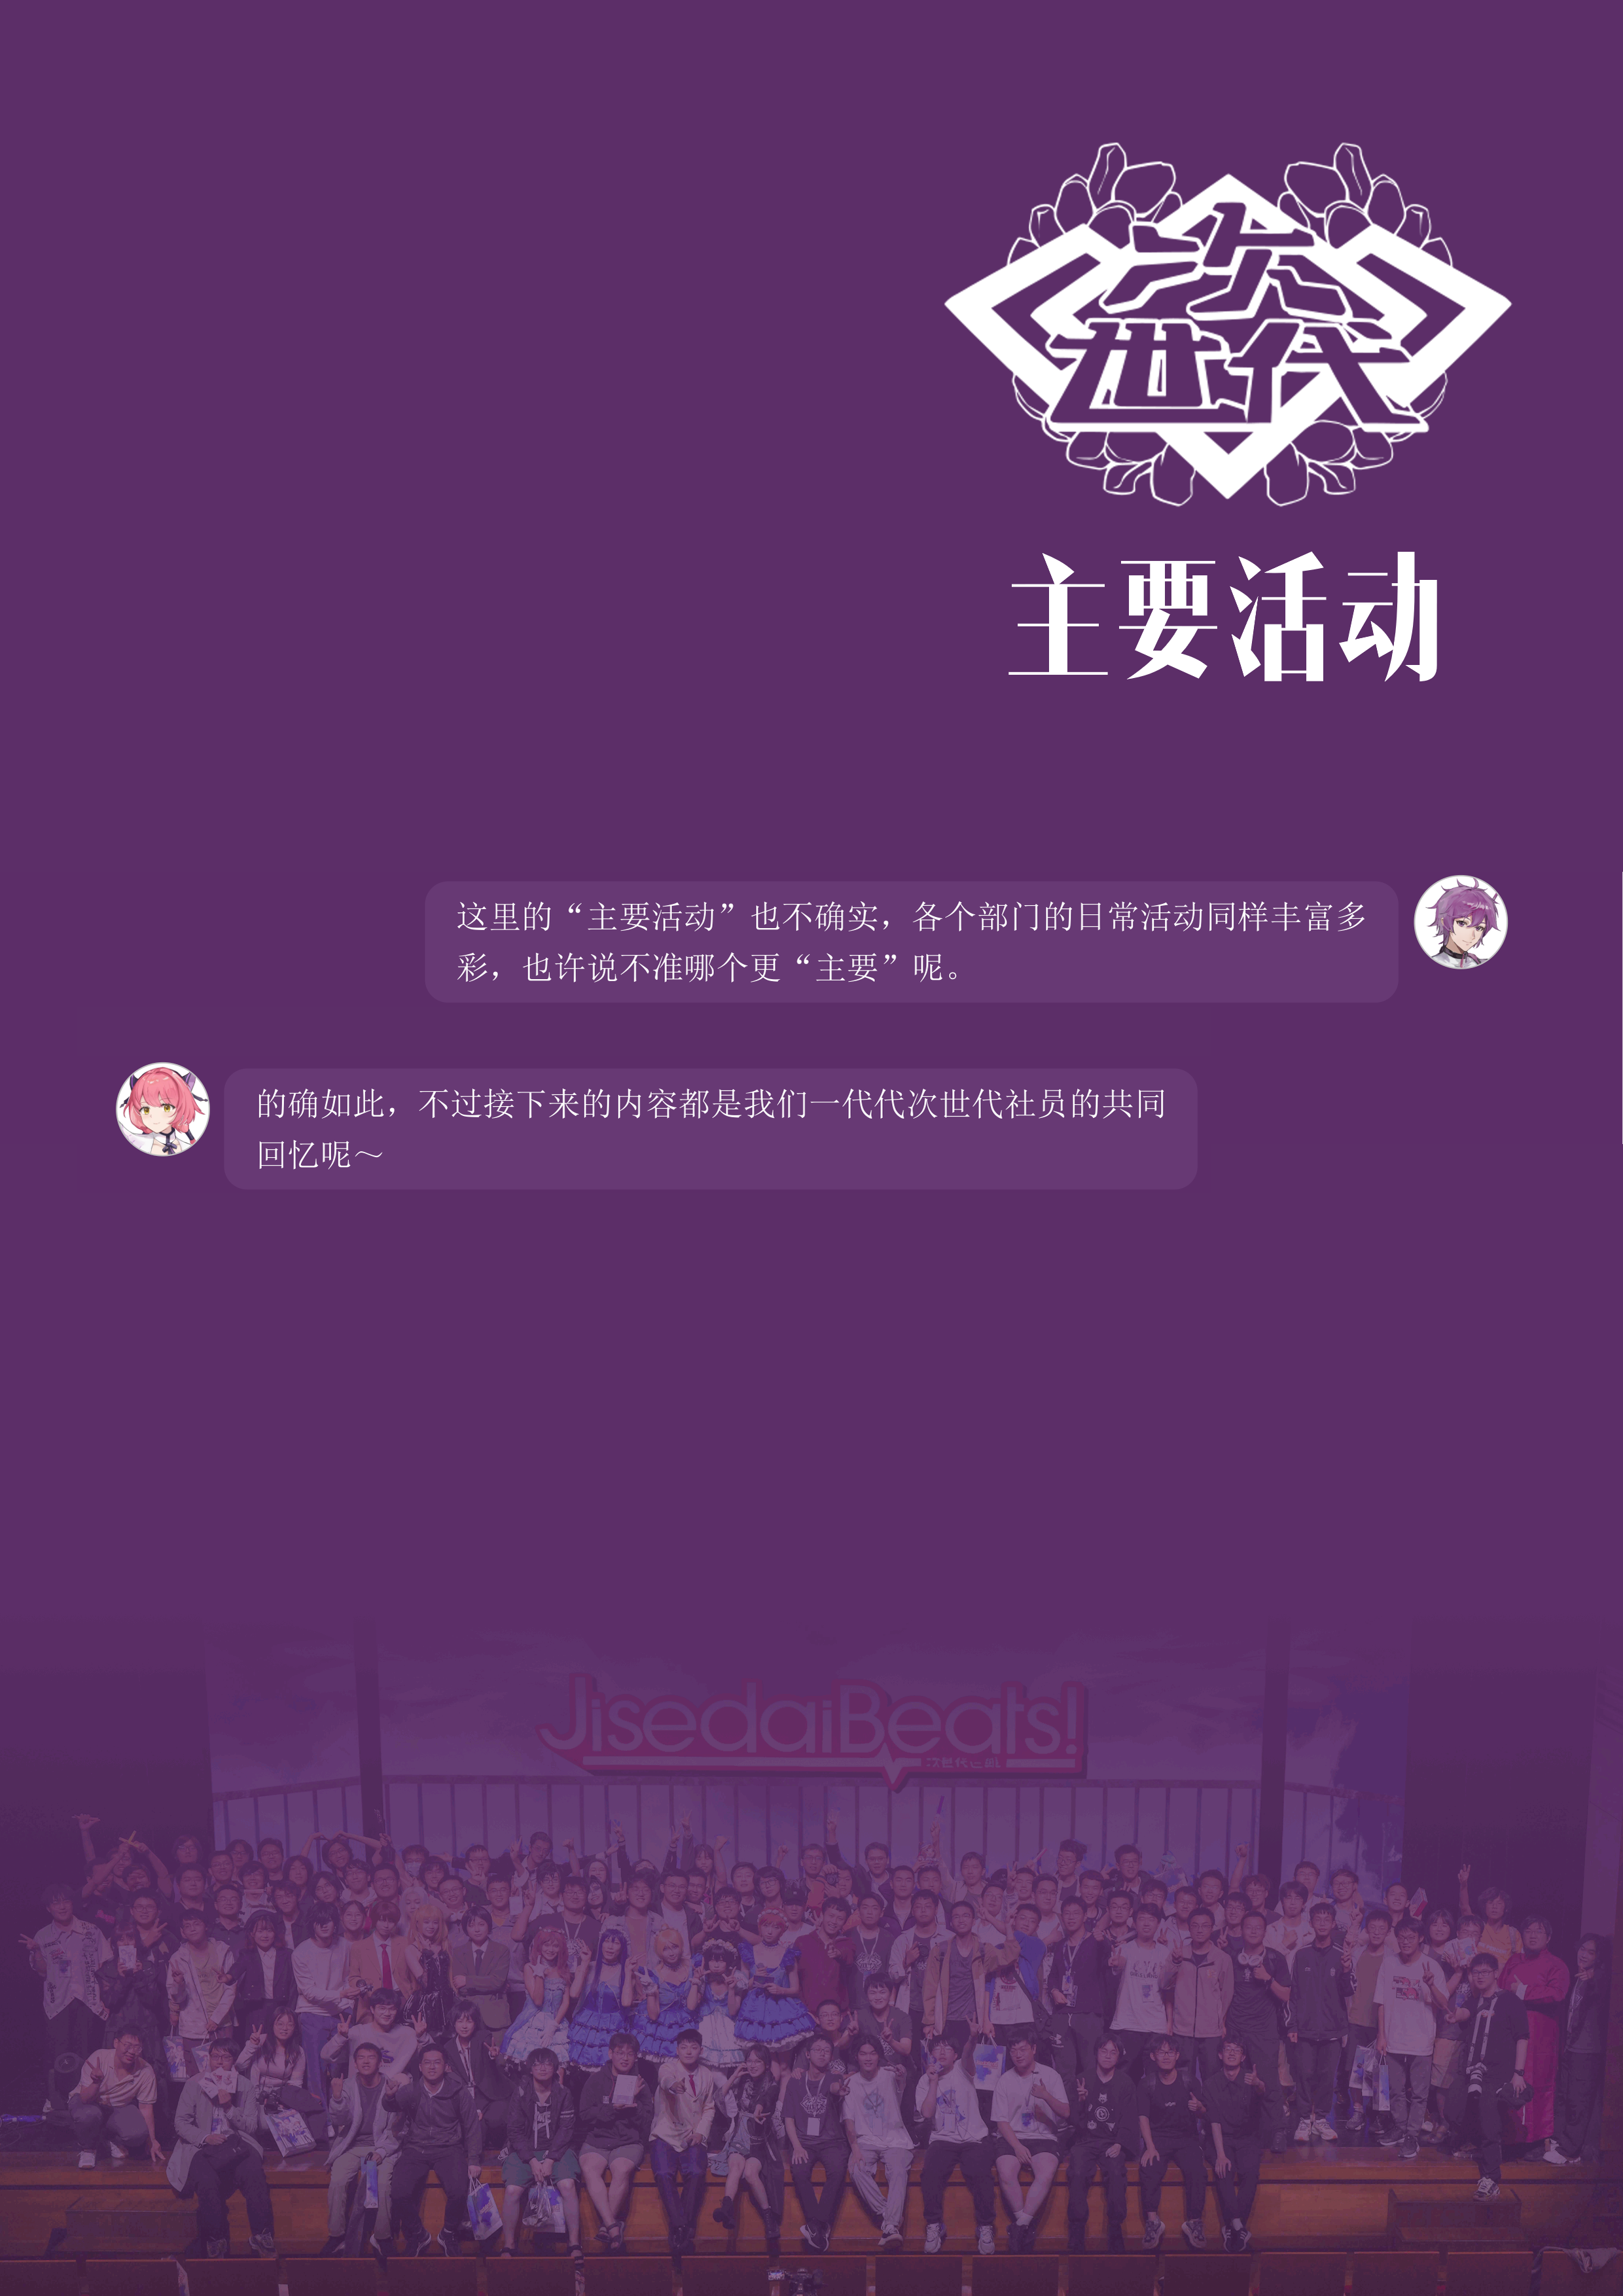
\includegraphics[width=0.9999\paperwidth, height=0.9999\paperheight]{ch2.png} % 插入图片,使其尺寸与纸张大小一致并保持宽高比[1](@ref)
    \restoregeometry % 恢复原来的页边距设置

\newpage
\newpage
\fontsize{23pt}{24pt}\selectfont
\textbf{\textcolor{truepurple}{百团大战\&迎新晚会}}\\
\vspace{0.7em}
\adjustbox{valign=t}{
	\begin{minipage}[t]{0.45\textwidth}
		\normalsize
		\chind 一年两度,次世代的大家拿出自己最大的热情欢迎新朋友!\\
    \chind 我们一直是百团最热闹的摊位之一。有各位同学自发贡献展示的手办、周边、图书展出;来自绘画部画师们的现场签绘、互绘;乐队部带来的现场演奏;cosplay舞台剧部的coser聚会、宅舞部献上的随舞表演;以及随后的wota艺节目……是招新,也是借机团建!\\
    \chind 在百团之后,我们会举办迎新晚会,进行各个分部的介绍展示与好玩的一站到底环节。\\
  		\par
		\vspace{-1em}
		\raisebox{-\height}{
			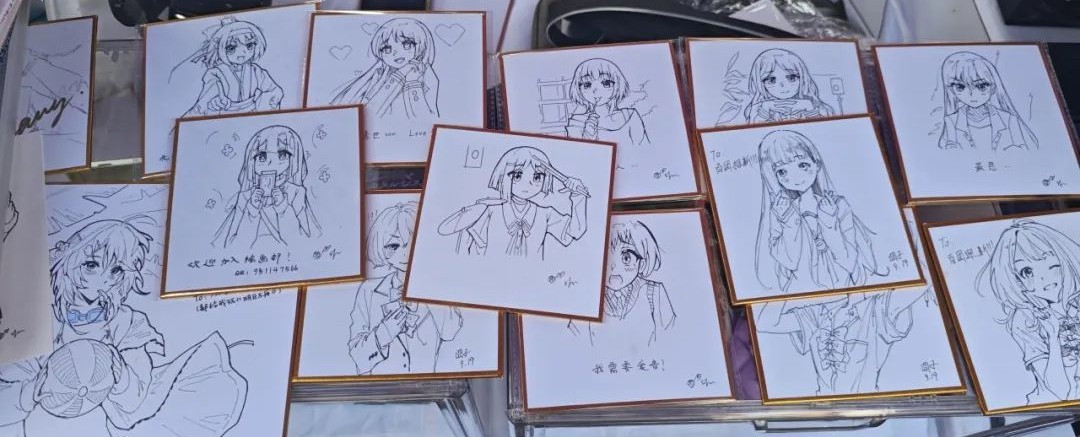
\includegraphics[width=\linewidth]{百团4.jpg}}
		\vspace{-0.5em}
		\picbox{\small ~\ding{115} ~ 绘画部现场签绘~}
		\par
		\vspace{-1em}
		\raisebox{-\height}{
			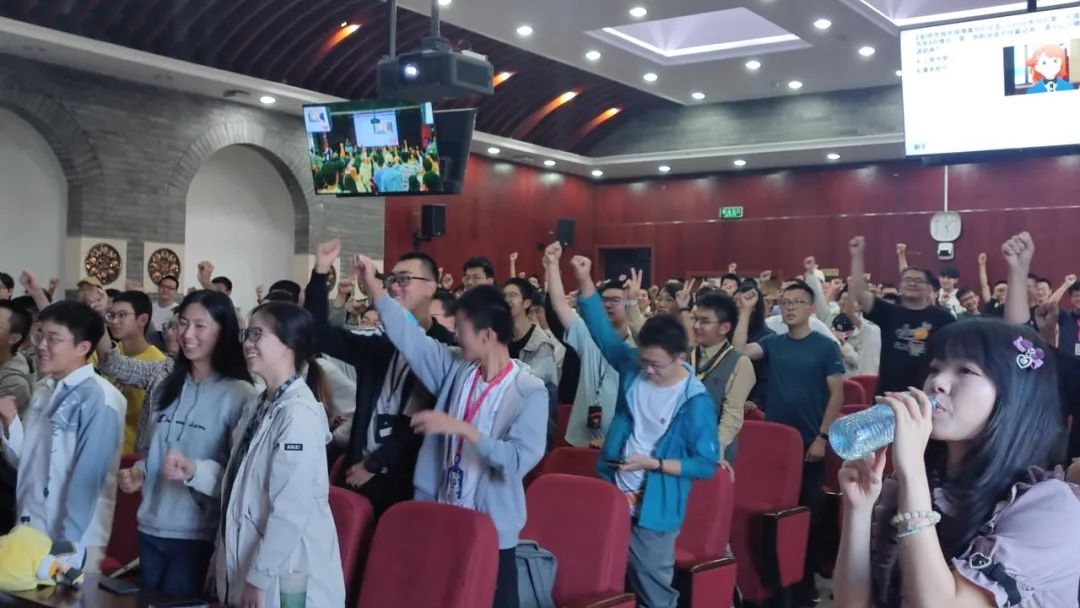
\includegraphics[width=\linewidth]{百团3.jpg}}
		\vspace{-0.5em}
		\picbox{\small ~\ding{115} ~ 一站到底~}
	\end{minipage}}
\hfill
\vspace{1em}
\adjustbox{valign=t}{
	\begin{minipage}[t]{0.45\textwidth}
		\vspace{-0.5em}
		\raisebox{-\height}{
			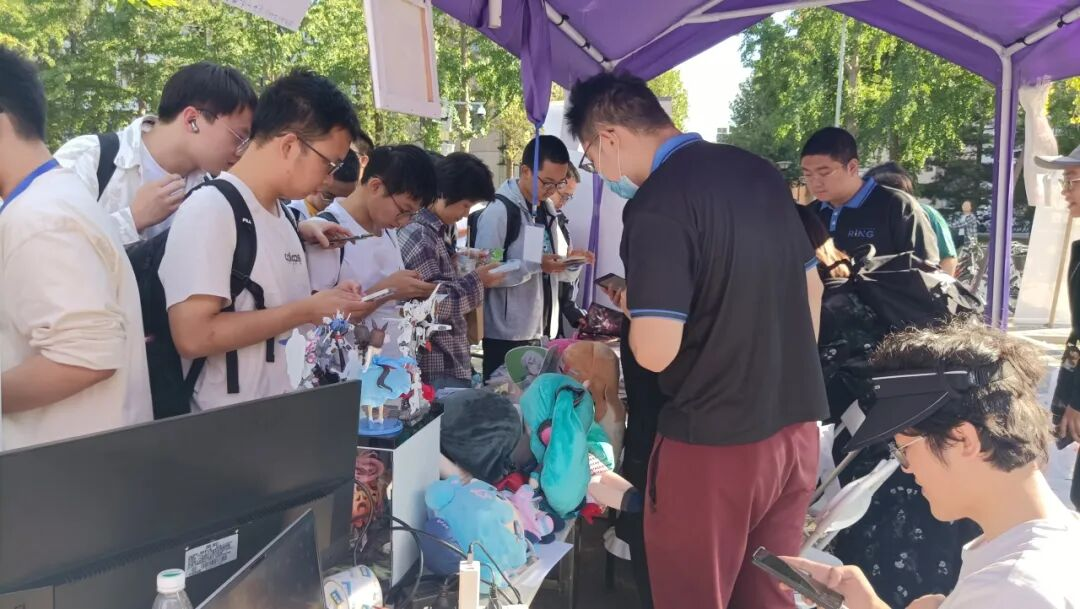
\includegraphics[width=\linewidth]{百团1.jpg}}
		\vspace{-0.5em}
		\picbox{\small ~\ding{115} ~ 走\sout{错}\textbf{对}大学第一步~}
		\par
		\vspace{-1em}
		\raisebox{-\height}{
			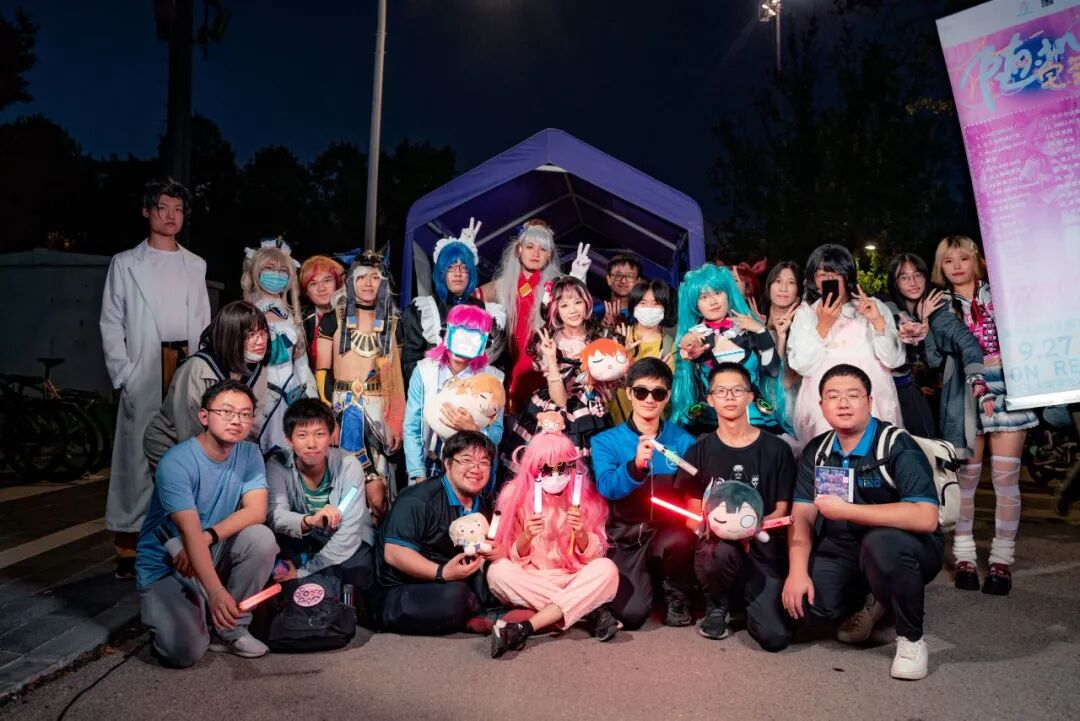
\includegraphics[width=\linewidth]{百团2.jpg}}
		\vspace{-0.5em}
		\picbox{\small ~\ding{115} ~ 随机宅舞~}
		\par
		\vspace{-1em}
		\raisebox{-\height}{
			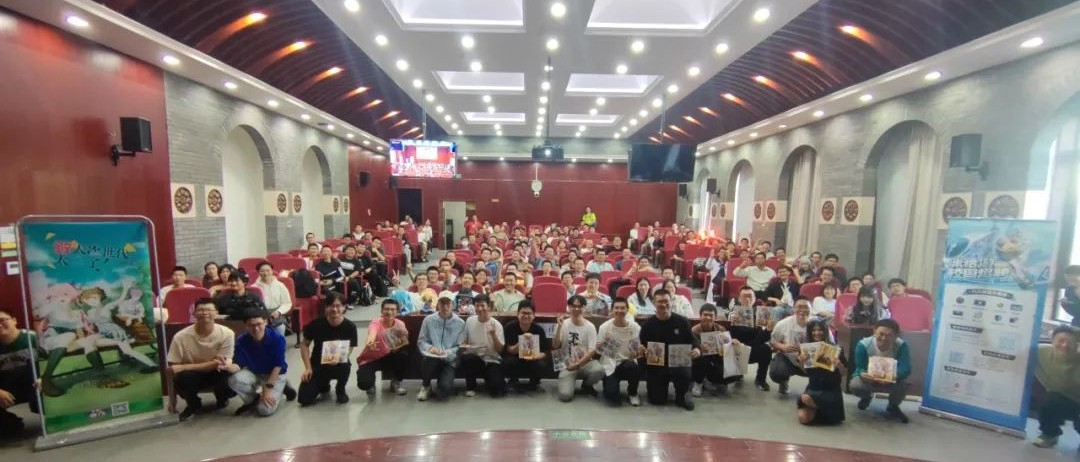
\includegraphics[width=\linewidth]{百团5.jpg}}
		\vspace{-0.5em}
		\picbox{\small ~\ding{115} ~ 迎新晚会合影~}
	\end{minipage}%
}
\begin{textblock*}{\paperwidth}(0mm, \dimexpr\paperheight-75mm\relax) % 距顶部 = 纸高 - 30mm
  \noindent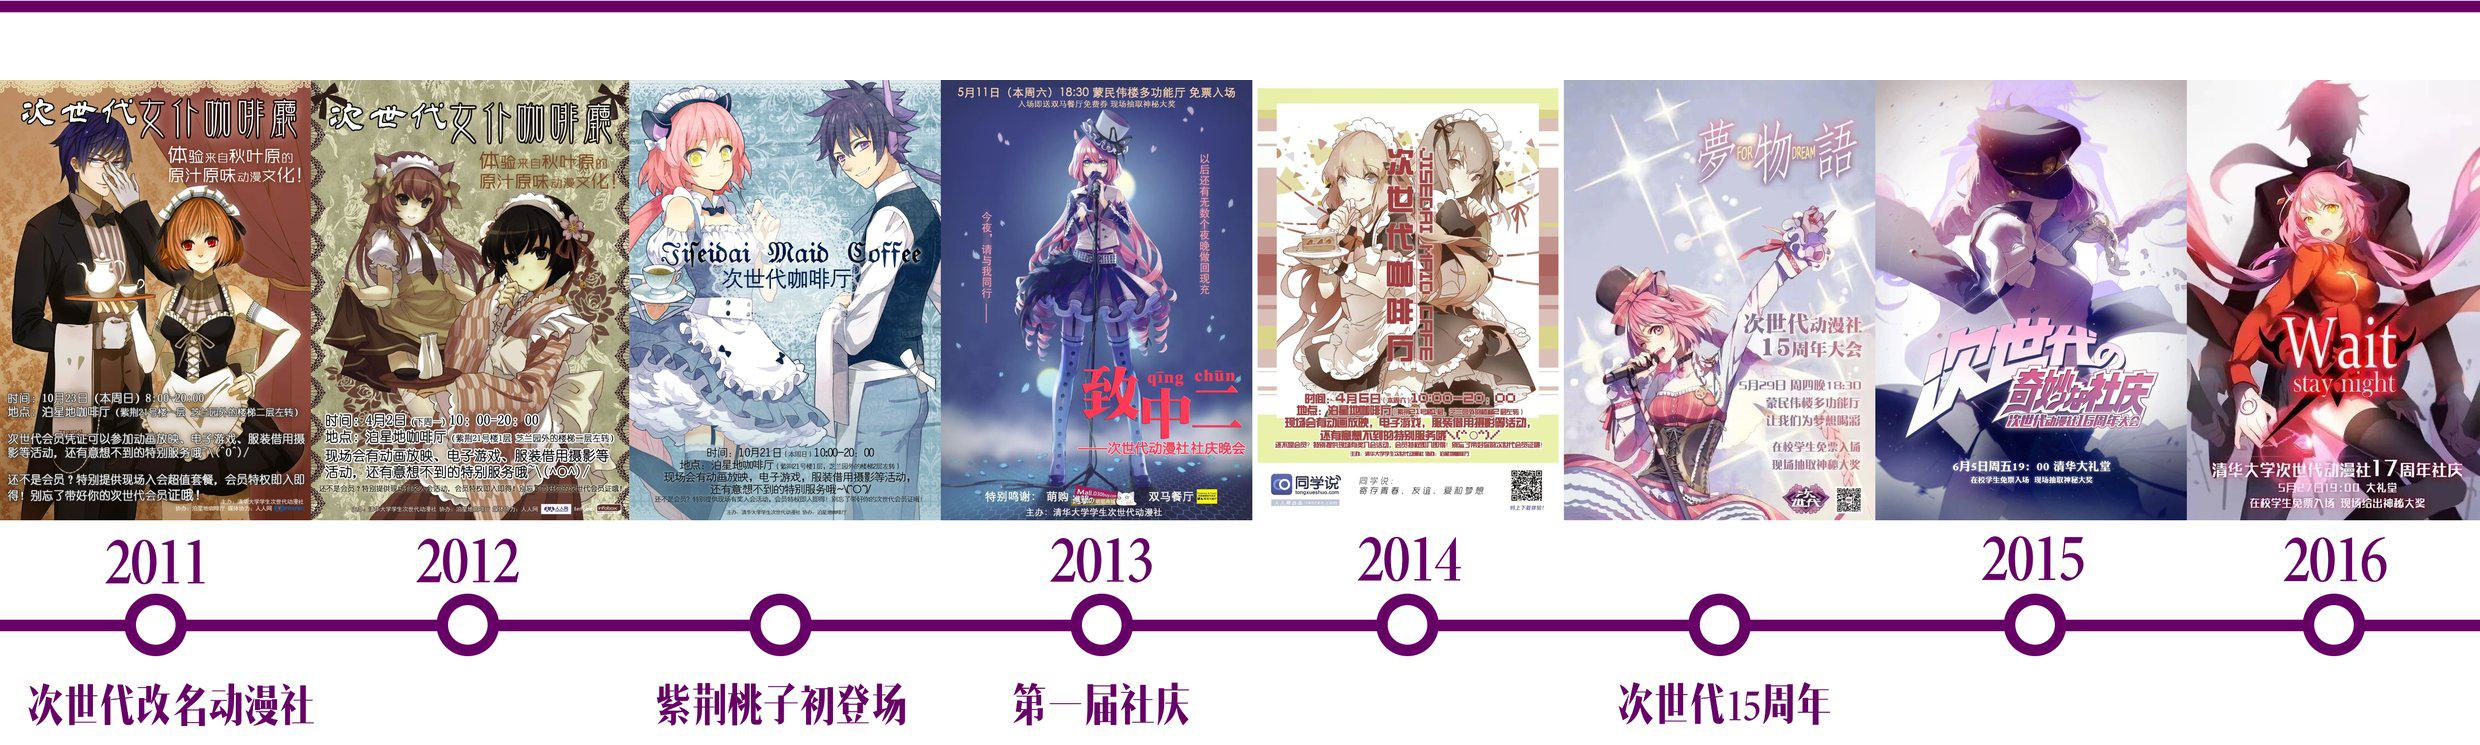
\includegraphics[width=\paperwidth]{tl1.jpg}
\end{textblock*}
\newpage
2
\begin{textblock*}{\paperwidth}(0mm, \dimexpr\paperheight-75mm\relax) % 距顶部 = 纸高 - 30mm
  \noindent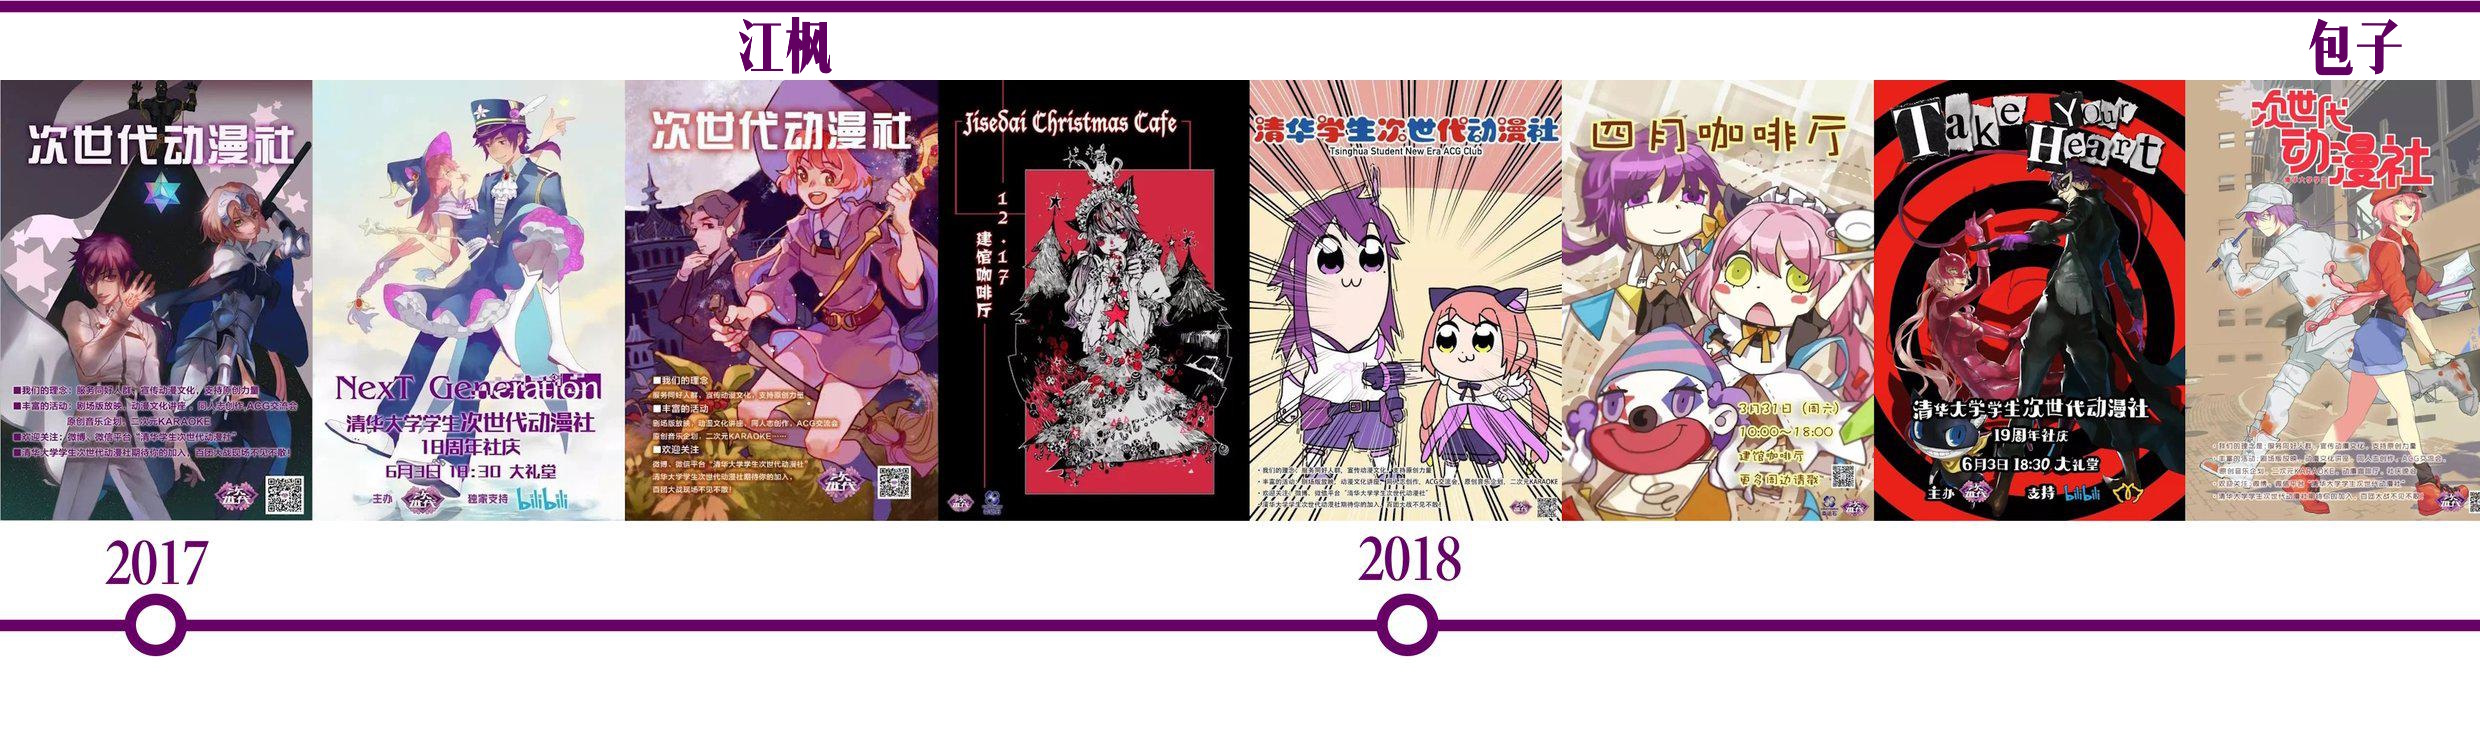
\includegraphics[width=\paperwidth]{tl2.jpg}
\end{textblock*}
\newpage
3
\begin{textblock*}{\paperwidth}(0mm, \dimexpr\paperheight-75mm\relax) % 距顶部 = 纸高 - 30mm
  \noindent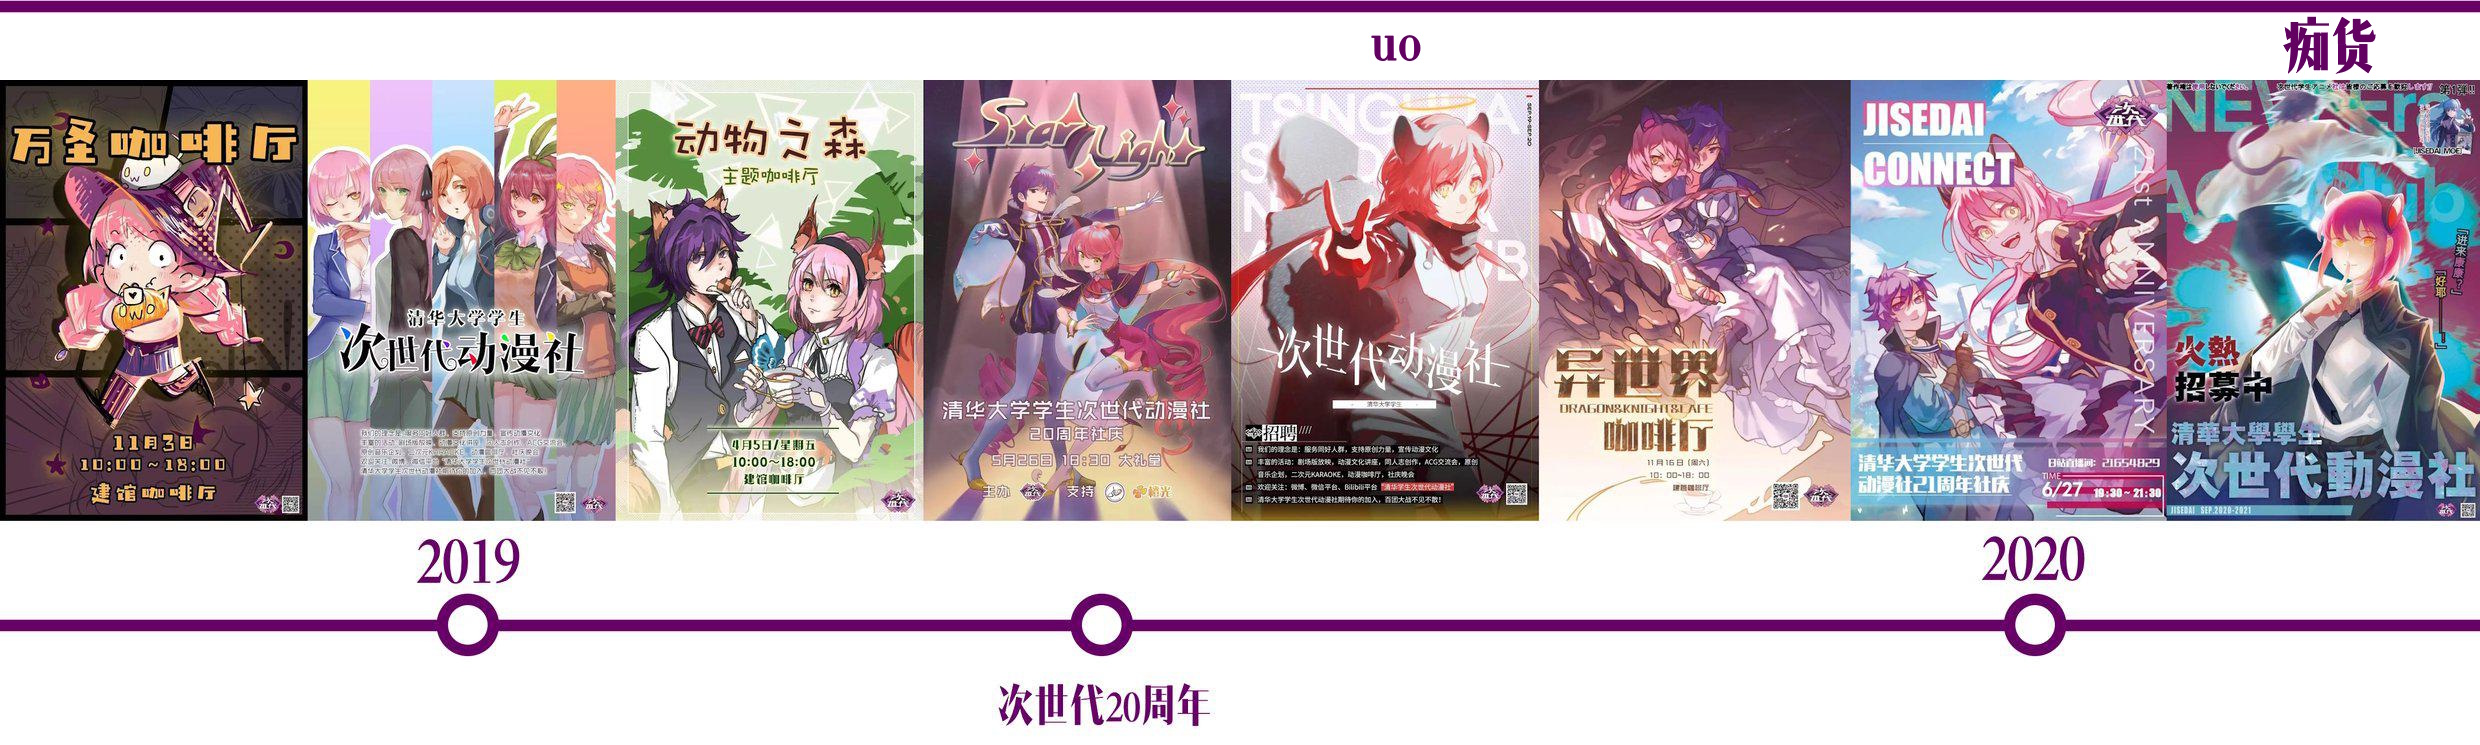
\includegraphics[width=\paperwidth]{tl3.jpg}
\end{textblock*}
\newpage
4
\begin{textblock*}{\paperwidth}(0mm, \dimexpr\paperheight-75mm\relax) % 距顶部 = 纸高 - 30mm
  \noindent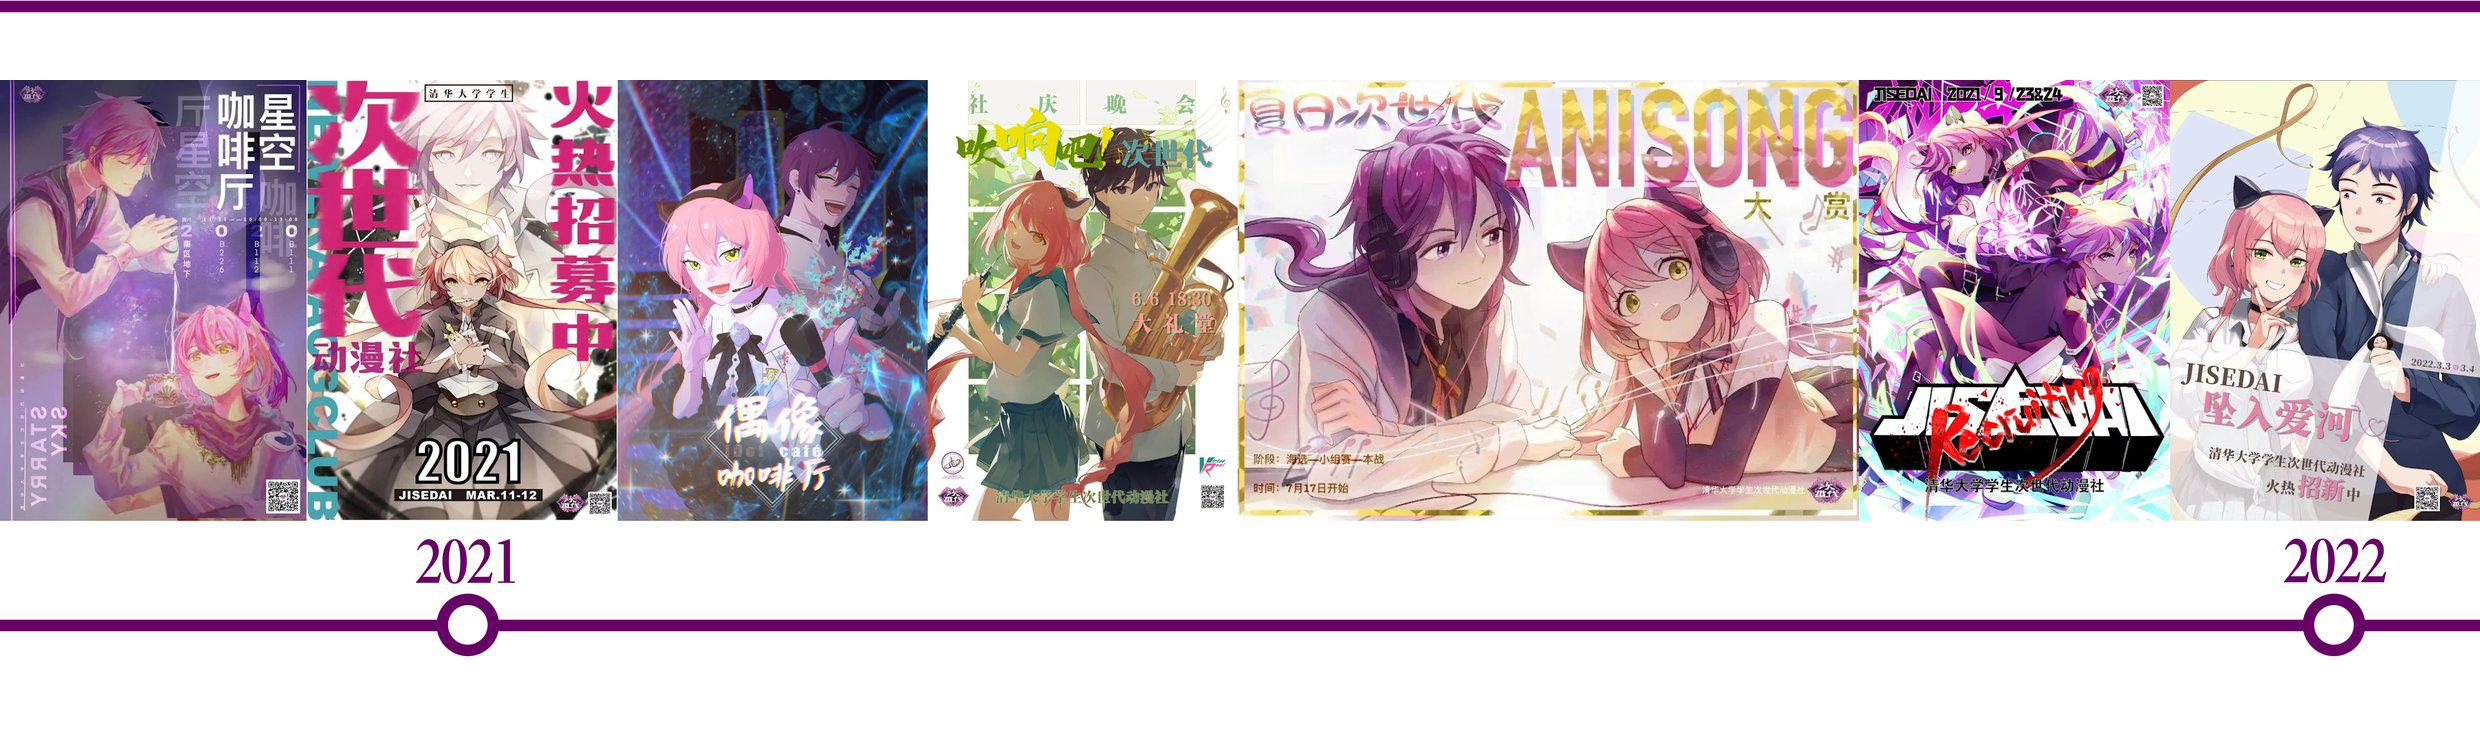
\includegraphics[width=\paperwidth]{tl4.jpg}
\end{textblock*}
\newpage
1
\begin{textblock*}{\paperwidth}(0mm, \dimexpr\paperheight-75mm\relax) % 距顶部 = 纸高 - 30mm
  \noindent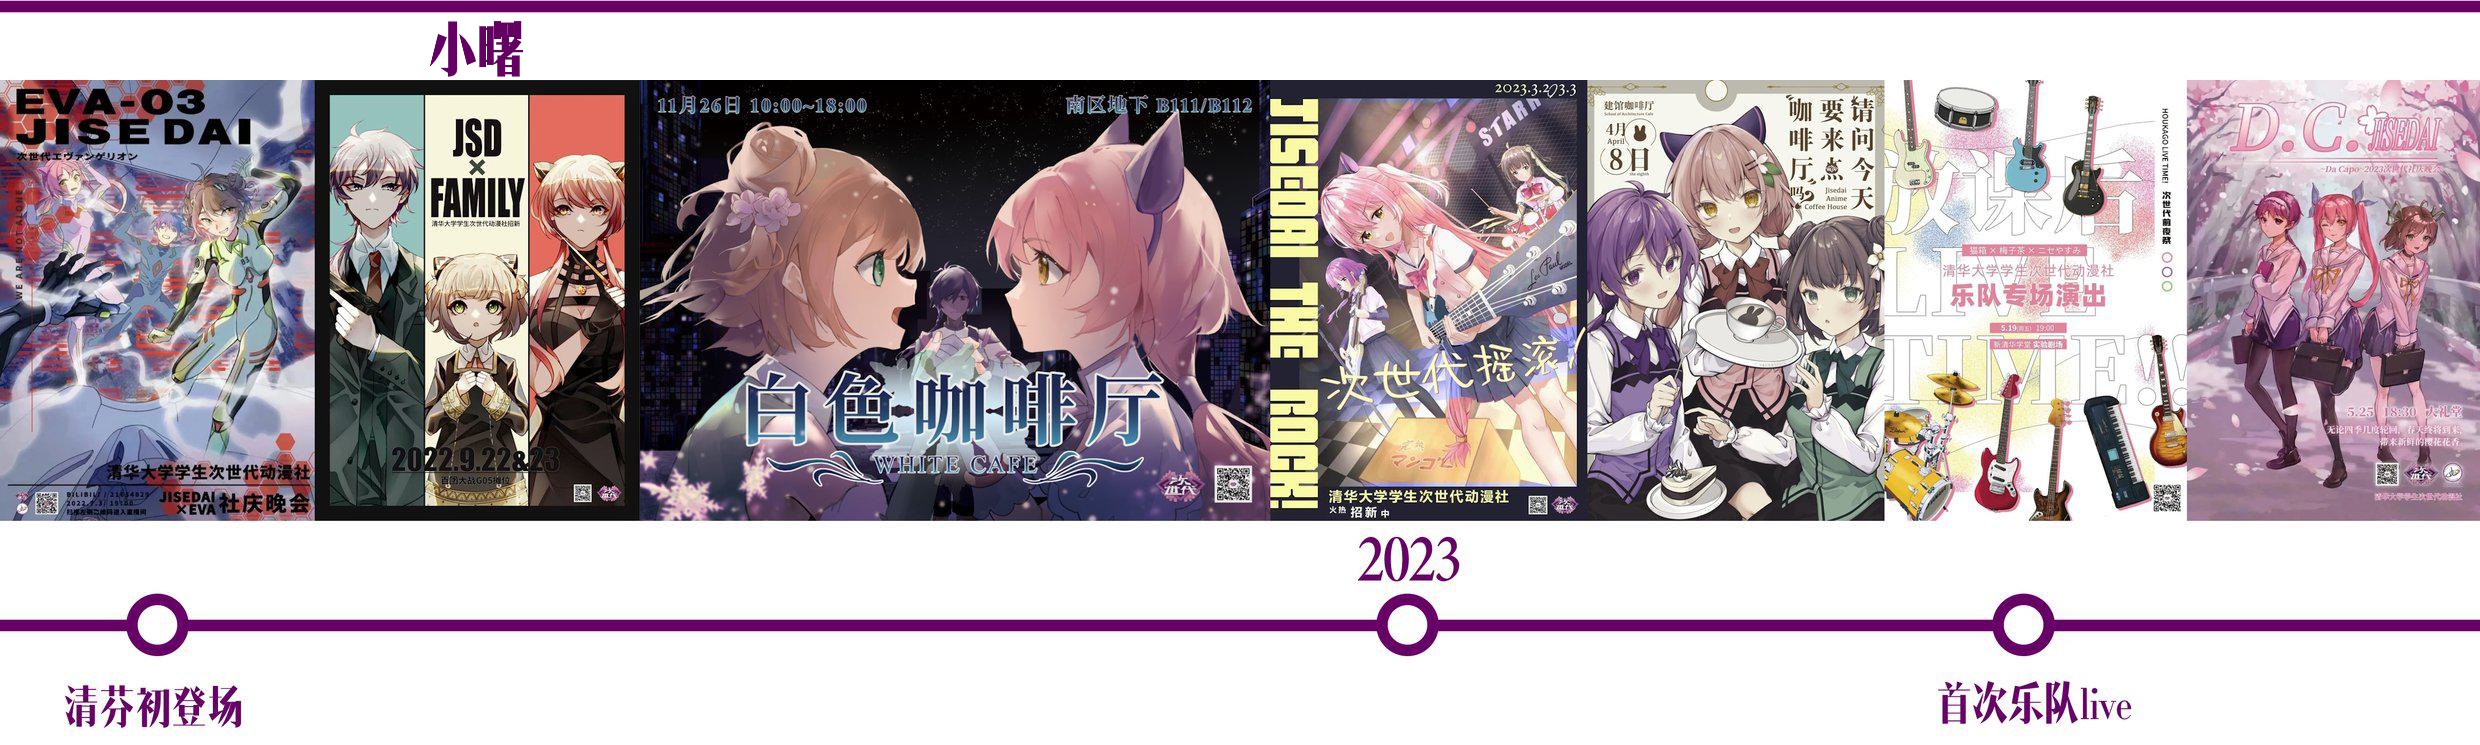
\includegraphics[width=\paperwidth]{tl5.jpg}
\end{textblock*}
\newpage
2
\begin{textblock*}{\paperwidth}(0mm, \dimexpr\paperheight-75mm\relax) % 距顶部 = 纸高 - 30mm
  \noindent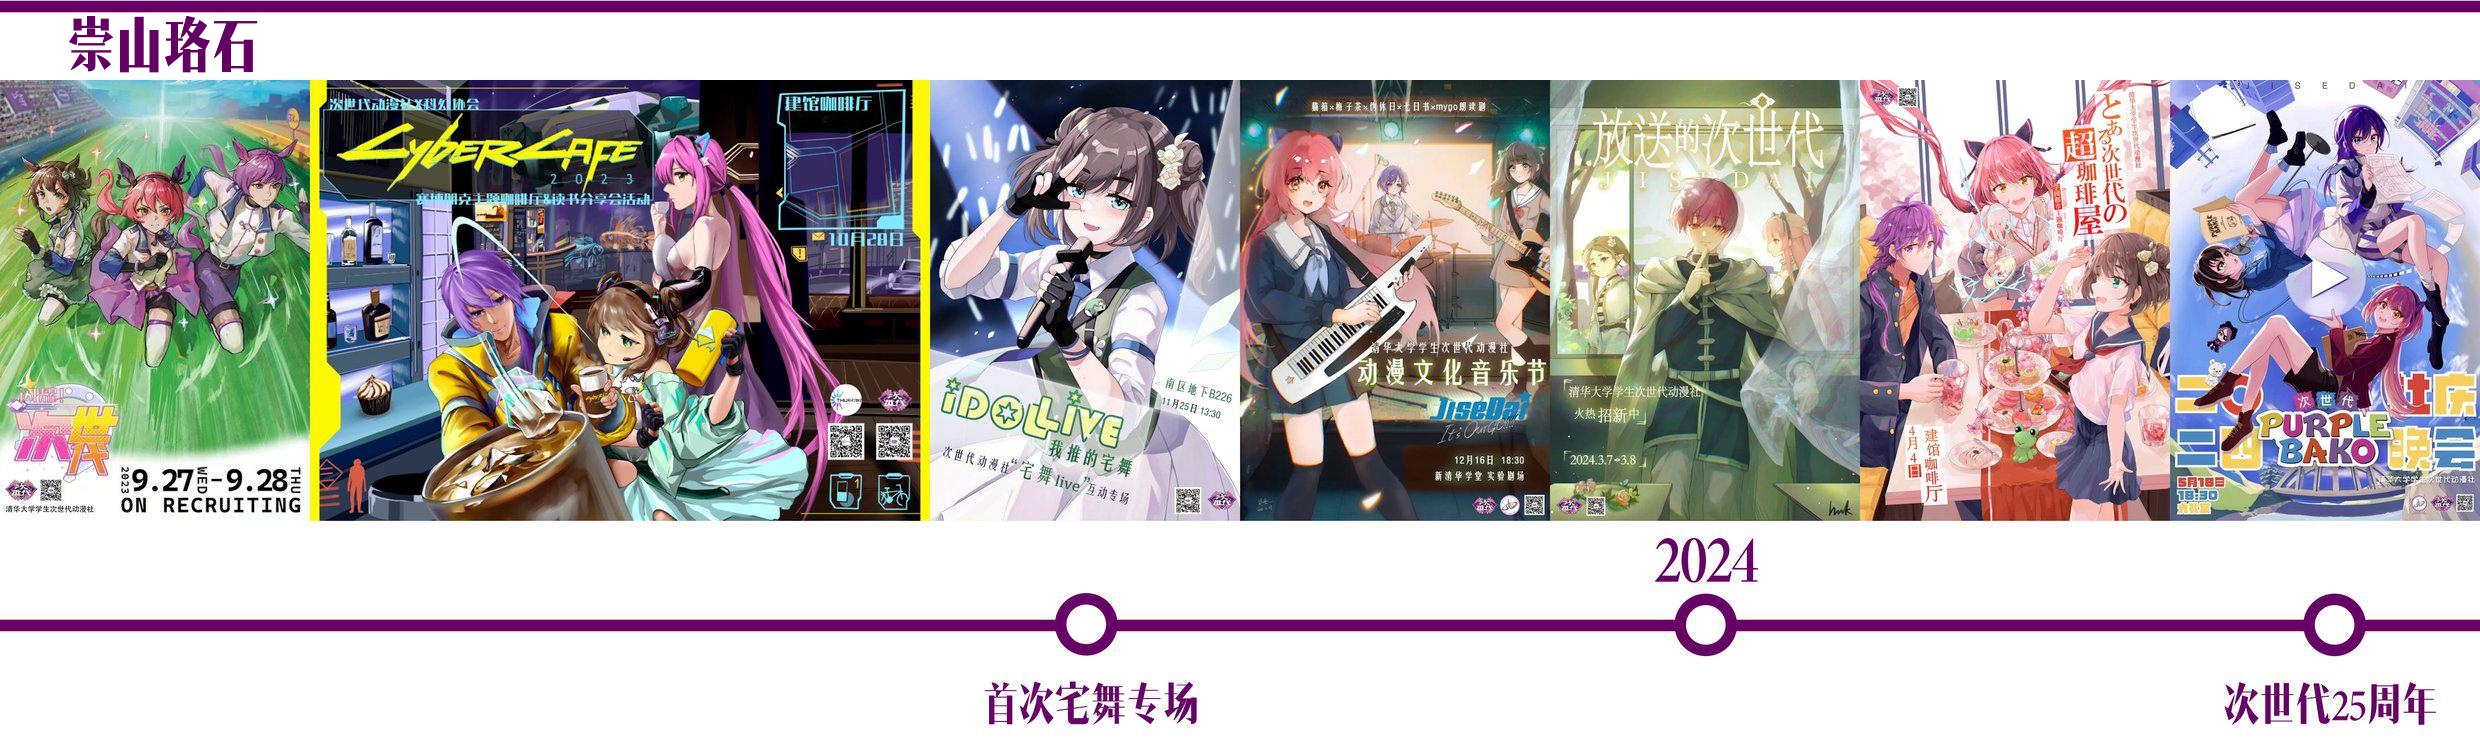
\includegraphics[width=\paperwidth]{tl6.jpg}
\end{textblock*}
\newpage
3
\begin{textblock*}{\paperwidth}(0mm, \dimexpr\paperheight-75mm\relax) % 距顶部 = 纸高 - 30mm
  \noindent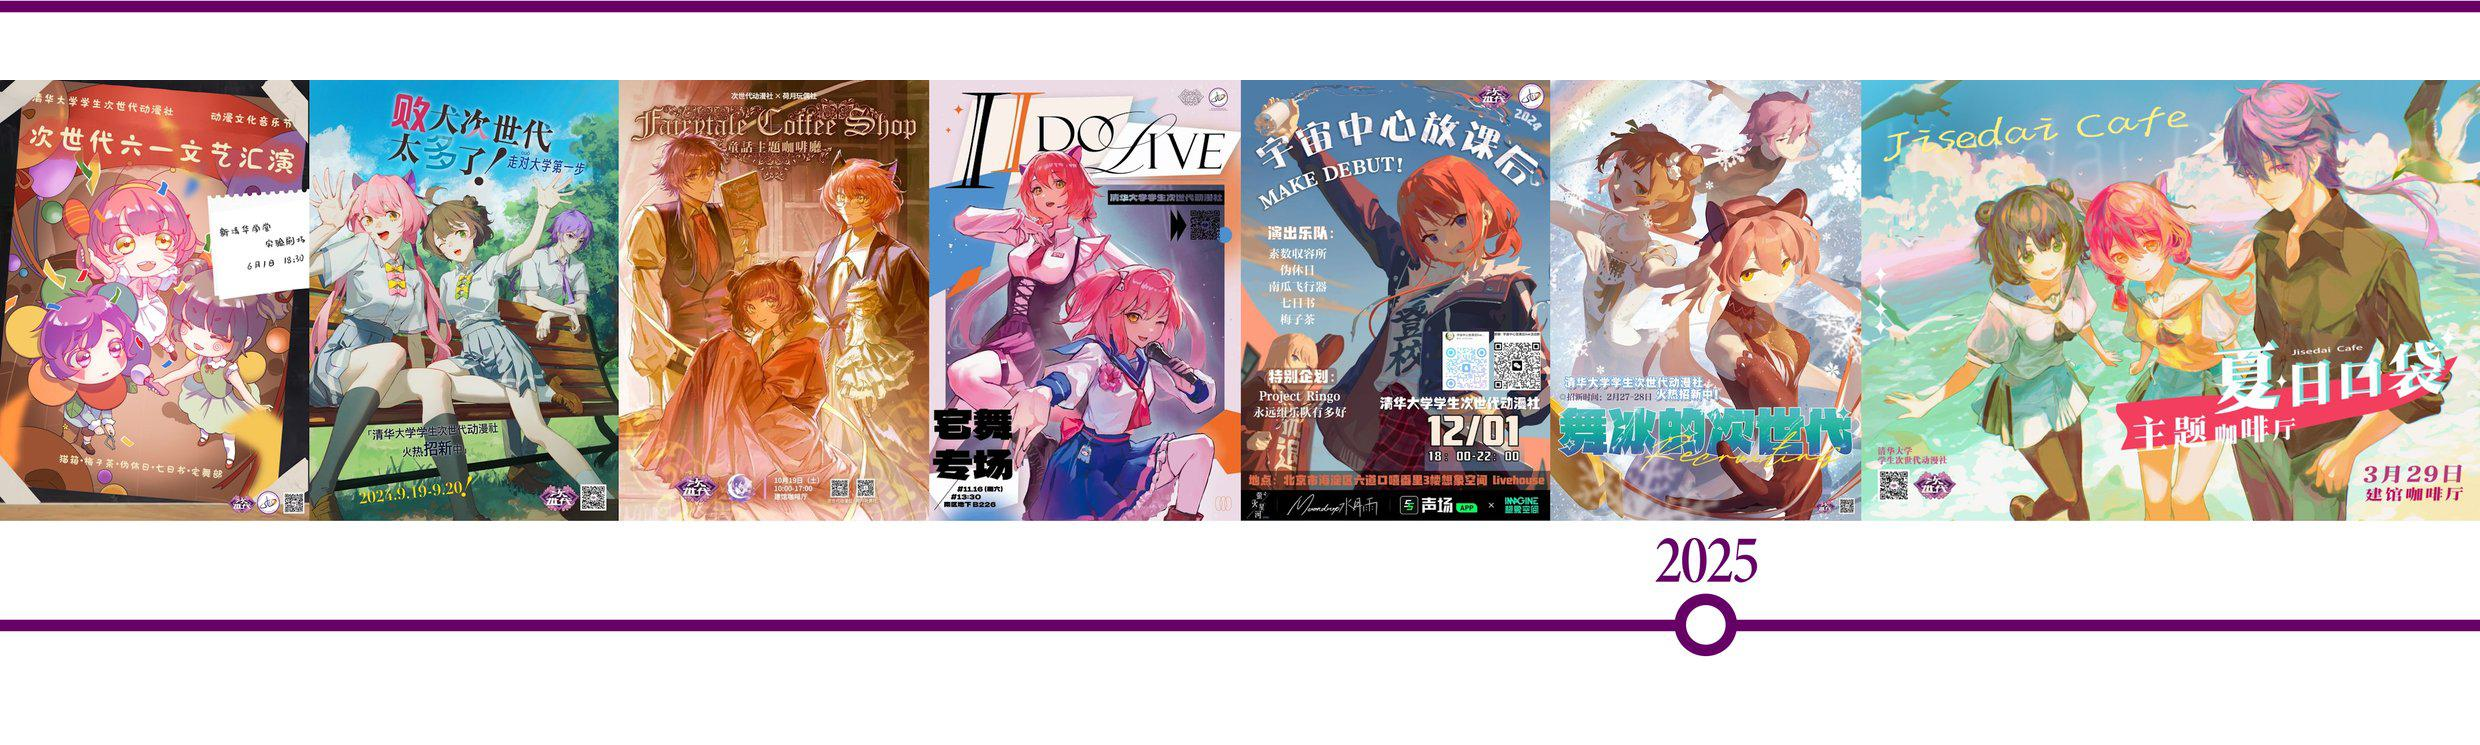
\includegraphics[width=\paperwidth]{tl7.jpg}
\end{textblock*}
\newpage
8
\begin{textblock*}{\paperwidth}(0mm, \dimexpr\paperheight-75mm\relax) % 距顶部 = 纸高 - 30mm
  \noindent
\includegraphics[width=\paperwidth]{tl8.jpg}
\end{textblock*}